% !TeX program = xelatex
% !TeX encoding = UTF-8
\documentclass[UTF8]{standalone}
\usepackage{amsmath,newtxmath,ctex,tikz}
\begin{document}
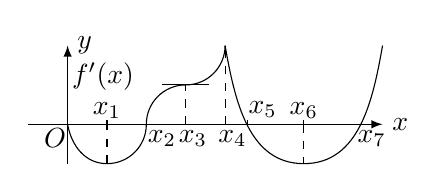
\begin{tikzpicture}
	\draw[-latex] (-0.5,0) -- (4,0) node[right] {$x$};
	\draw[-latex] (0,-0.5) -- (0,1) node[right] {$y$};
	\node at (0.45,0.6) {$f'(x)$};
	\draw (0,0) to[out=-80,in=-180] ++ (0.5,-0.5);
	\draw (0.5,-0.5) to[out=0,in=-90] ++ (0.5,0.5);
	\draw (1,0) to[out=90,in=-180] ++ (0.5,0.5);
	\draw (1.5,0.5) to[out=0,in=-90] ++ (0.5,0.5);
	\draw (1.5,0.5) ++ (-0.3,0) -- ++ (0.6,0);
	\draw (2,1) to[out=-80,in=-180] ++ (1,-1.5);
	\draw (3,-0.5) to[out=0,in=-100] ++ (1,1.5);
	\draw[dashed] (0.5,-0.5) -- ++(0,0.5);
	\draw[dashed] (1.5,0) -- ++(0,0.5);
	\draw[dashed] (2,0) -- ++(0,1);
	\draw[dashed] (3,0) -- ++(0,-0.5);
	\draw (0.5,0) -- ++ (0,0.05) node[above=-3pt] {$x_1$};
	\node[below=5pt,right=-3pt] at (1,0) {$x_2$};
	\node[below=5pt,right=-6pt] at (1.5,0) {$x_3$};
	\node[below=5pt,right=-6pt] at (2,0) {$x_4$};
	\draw (2.28,0) -- ++ (0,0.05) node[above=4pt,right=-3pt] {$x_5$};
	\draw (3,0) -- ++ (0,0.05) node[above=-3pt] {$x_6$};
	\node[below=5pt,right=-4pt] at (3.7,0) {$x_7$};
	% \fill (-1.5,0) circle (0.04) node[below=4pt,right=-3pt] (a) {$x_2$};
	% \draw[dashed] (-1.5,0) -- (-1.5,0.45);
	% \fill (-1.9,0) circle (0.04) node[below=4pt,right=-3pt] {$x_1$};
	\node[below=5pt,left=-3pt] at (0,0) {$O$};
	% \draw (-2,-0.5) to[out=80,in=-180] (-1.5,0.45);
	% \draw (-1.5,0.45) to[out=0,in=-180] (-1,0);
	% \draw (-1,0) to[out=0,in=-95] (-0.15,1.2);
\end{tikzpicture}
\end{document}